\documentclass[11pt]{article}
\usepackage[margin=1in]{geometry}
\usepackage{amsmath,amssymb,amsfonts}
\usepackage{graphicx,float}
\usepackage{fancyhdr,booktabs}
\usepackage{listings}
\usepackage{hyperref}
\usepackage{listings, soul}
\usepackage[most]{tcolorbox}
\tcbset{breakable}
\usepackage{tikz}
\usetikzlibrary{arrows.meta, positioning, calc}

\lstset{
    language=Matlab,
    basicstyle=\ttfamily\small,
    breaklines=true,
    keepspaces=true,
    showstringspaces=false
}


\title{\textbf{ME 352 QUBE Motor Freq Design}\\[0.5ex]\Large Final Workshop}
\author{Zeshui Song}
\date{Fall 2026}

\begin{document}
\maketitle
\vspace{-1em}
\section*{Part 1: Speed Controller}
\section*{Second Order Transfer Function of QUBE Motor}
Speed control:
\[\boxed{G(s) = \frac{\Omega (s)}{V(s)} = \frac{k_m}{JLs^2 + (JR+BL)s+(BR + k_mk_b)}}\]
\subsection*{Problem 1:} 
Bode plot of open loop motor system:
\begin{center}
    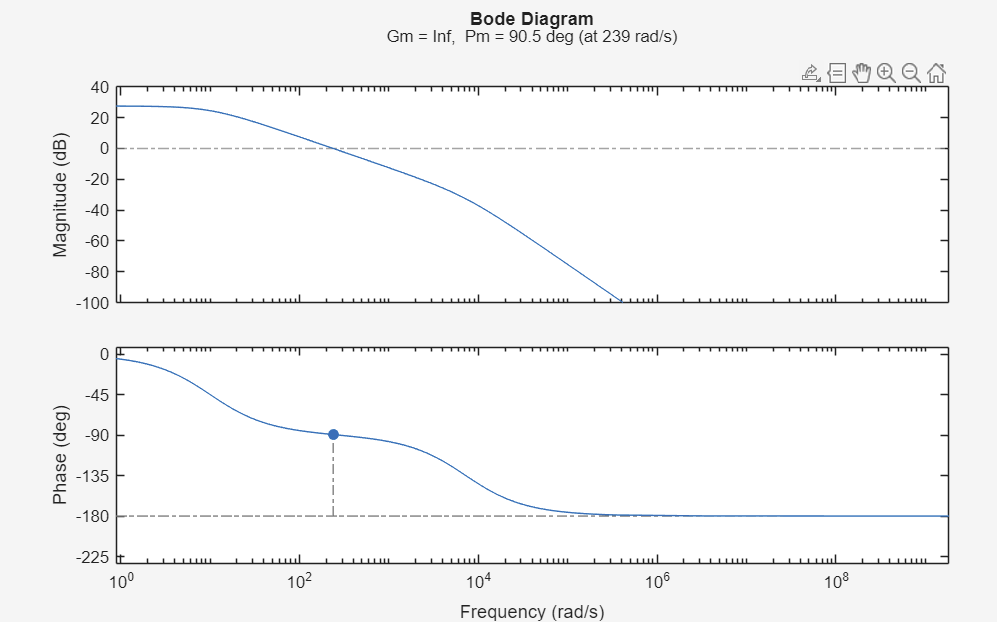
\includegraphics[width = 0.8\textwidth]{OL Bode.png}
\end{center}
\subsection*{Problem 2:}
Gain margin is infinite which means that we can theoretically increase the controller gain to infinity without making the system unstable (never reaches phase = -180 deg and magnitude = 0 dB).
\subsection*{Problem 3:}
The phase margin is 90.5 degrees which means that the open loop system is pretty stable.
\subsection*{Problem 4:}
Bandwidth is 10.0146 rad/s for the open loop system.
\subsection*{Problem 5:}
The crossover frequency is 238.6701 rad/s for the open loop system.
\subsection*{Problem 6:}
Since zeta = 13.441 so the open loop system is \textbf{overdamped}.
\subsection*{Problem 7:}
The open loop system is overdamped so there would be two real poles. These two poles correspond to two different time constants:
\[\tau_1 = -\frac{1}{s_1}=1.3829\times10^{-4}\]
\[\tau_2 = -\frac{1}{s_2}= 0.0996\]
\subsection*{Problem 8:}
The open loop poles are at:
\[s_1 = -7231.3408,\quad s_2 = -10.0385\]
The pole closest to the origin is $s_2 = -10.0385$ which corresponds to the dominant time constant $\tau_2 = 0.0996$.
\subsection*{Problem 9:}
\begin{center}
    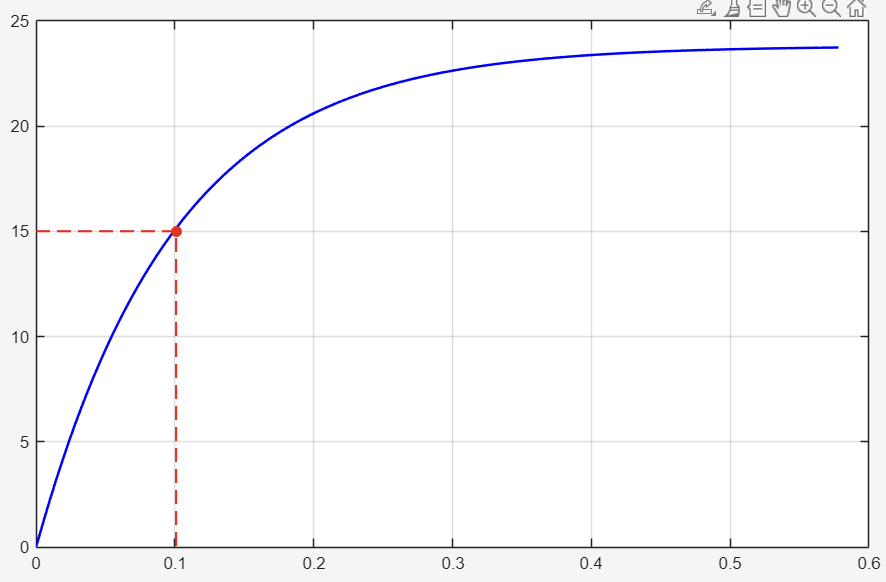
\includegraphics[width=0.6\textwidth]{OL step response.png}
\end{center}
The estimated time constant from the step response (time to reach 63.2\% of the final value) is $\tau = 0.1009$ seconds. This is very close to the calculated dominant time constant $\tau_2 = 0.0996$ seconds.
\subsection*{Problem 10+11:}
By looking at the root locus plot, the system is critically damped when both poles are at the same location on the real axis. This occurs when the gain is $K = 7.54$
\subsection*{Problem 12:}
The steady state error for a unit step input is 0.0055.
\subsection*{Problem 13:}
The steady state error for a unit ramp input is infinite.
\subsection*{Problem 14:}
The closed loop phase margin is 76.7132 degrees.
\subsection*{Problem 15:}
While we can theoretically accept high gains, the model we use doesn't include other system effects such as noise. Thus, by increasing gain, these unmodeled effects can become significant and cause the system to behave in unintended ways.
\newpage
\section*{Part 2: Servo position controller}
\subsection*{Problem 16:}
The bode plot of the open loop position control loop transfer function is shown below:
\begin{center}
    \includegraphics[width=0.8\textwidth]{OL Bode position.png}
\end{center}
\subsection*{Problem 17:}
Open loop nyquist plot for the position plant is shown below:
\begin{center}
    \includegraphics[width=0.8\textwidth]{OL Nyquist.png}
\end{center}
\subsection*{Problem 18:}
The gain margin is 49.7 dB.
\subsection*{Problem 19:}
The phase margin is 35.7 degrees.
\subsection*{Problem 20:}
For a phase margin of 60 degrees, we would want a crossover gain of 5.67 rad/s. Thus, we will need to decrease the gain of the system to shift magnitude plot down so that the crossover frequency is lower.
\end{document}
